% !TEX root = ../../main.tex
% !TEX encoding = UTF-8 Unicode
% !TEX encoding = UTF-8

\chapter{Kosten und Zeit - BB, SH, KL}

In diesem Kapitel werden Informationen \"uber Kalkulationen der Kosten und Methoden der Zeitplanung gegeben. Die gew\"ahlten Projekte Alfresco, Responsive Webdesign und Facebook-Tabs sind als Vorlagen zu betrachten, da die Vorgehensweisen auch auf andere Anforderungen, die diese Arbeit nicht betrachtet, angewendet werden k\"onnen. Die Methoden wurden im Hinblick auf die Besonderheiten der Hochschule Emden/Leer ausgew\"ahlt. Am Ende des Kapitels werden ausgew\"ahlte Projekte vorgestellt, die der vorgeschlagenen SOLL-Situation \"ahnlich sind bzw. vergleichbare Systeme in ihrer Umsetzung, f\"ur ein integriertes Informationsmanagement, errichten konnten.

\section{Kostenarten}
\label{section_kostenarten}
Kalkulationen benötigt bestimmte eindeutige Kostenarten, die dann in einem Kostenartenplan aufgestellt und in einer Kostenartenrechnung kontrolliert werden können. Die eindeutige Kostenarten können in Kostenartenkategorien bzw. Kostenartengruppen zusammen fließen.  Im folgenden soll einmal festgehalten werden, was man für die Kalkulation nutzen sollte.

\begin{figure}[h!]
	\centering
	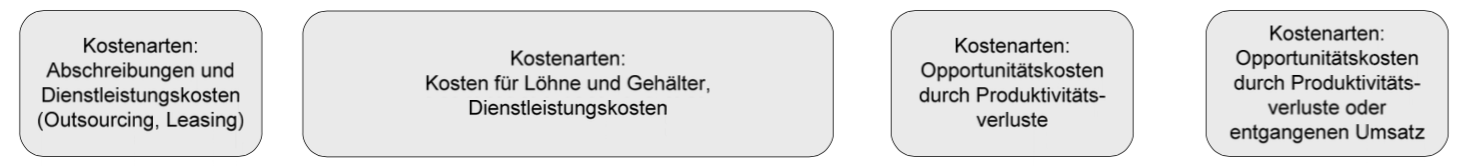
\includegraphics[width=\textwidth]{kapitel/gruppe4_2/bilder/beispiel_kostenarten_TCO}
	\caption{Beispiel von Kostenarten in der TCO-Methode, Grafik von Hansen}
	\label{fig_kostenarten_TCO}
\end{figure}

In der Abbildung \ref{fig_kostenarten_TCO} nach Hansen\footnote{\cite{hansen_business_2009}} finden sich z.B. in der von Krcmar benannten TCO-Methode (“Total Cost of Ownership”) wieder. Aus den bewerteten Daten der Kostenarten können periodische Durchschnittswerte ermittelt werden, aus denen dann für die Zukunft neue Abschätzungen gewonnen werden.

In einer ABC-Analyse kann eine weitere Klassifizierung vorgenommen werden, um z.B. aufzuzeigen welche Kostenarten auf jeden Fall (A-Klasse) anfallen, welche im besten Fall noch erledigt werden sollen (B-Klasse) und welche man optional (C-Klasse) aufwenden sollte.

Die Kostenarten in der Tabelle \ref{tab_gliederung_kostenarten} sind die Grundelemente der Wertsteigerung durch Wertschöpfung, die in die Kostenartenrechnung fließen sollten. „Die Kostenartenrechnung erfasst, systematisiert und periodisiert die Kosten.“\footnote{\cite{reim_erfolgsrechnung_2015}} 

Die Kostenarten in der Tabelle \ref{tab_gliederung_kostenarten} sollen in diesem Projekt als Übersicht dienen, da aktuell nur drei Module in der Kostenschätzung betrachtet werden, für den Fall das weitere Module abzuschätzen sind.

\begin{table}[h!]
\begin{tabularx}{\textwidth}{|X|X|}
	\hline \textbf{Gliederungsmerkmale nach}  &  \textbf{Kostenartengruppen}\\ 
	\hline der Zahlungswirksamkeit  & \begin{itemize}
		\item Grundkosten
		\item kalkulatorische Kosten
	\end{itemize} \\ 
	\hline der Art der verbrauchten Einsatzgüter & \begin{itemize}
		\item Materialkosten
		\item Personalkosten
		\item Fremdleistungskosten
		\item (Kalkulatorische) Abschreibungen
		\item (Kalkulatorische) Kapitalkosten
		\item Kalkulatorische Zusatzkosten
		\item Kostensteuern und Gebühren
	\end{itemize} \\ 
	\hline der Herkunft der verbrauchten Einsatzgüter & \begin{itemize}
		\item Primäre Kosten
		\item Sekundäre Kosten	
	\end{itemize}  \\ 
	\hline den Funktionsbereichen &\begin{itemize}
		\item Beschaffungskosten
		\item Fertigungskosten
		\item Vertriebskosten
		\item Forschungs- u. Entwicklungskosten
		\item Verwaltungskosten
	\end{itemize} \\ 
	\hline der Beschäftigungsabhängigkeit & \begin{itemize}
		\item Variable Kosten
		\item Fixe Kosten
	\end{itemize} \\ 
	\hline der Art der Verrechnung & \begin{itemize}
		\item Einzelkosten
		\item Gemeinkosten
		\item Sondereinzelkosten
	\end{itemize} \\ 
	\hline 
\end{tabularx}
	\caption{Gliederungsmöglichkeiten der Kostenarten, nach Reim}
	\label{tab_gliederung_kostenarten}
\end{table}

\subsection{Kostenarten in Hochschulen}
Im Hochschulbereich betrachtet man besonders die Kostenarten der Einzelkosten und Gemeinkosten. Die Kostenarten müssen, im universitären Umfeld, besonders in Forschungsprojekten mit Drittmitteln genau aufgeschlüsselt und zugewiesen werden, um einen transparenten Überblick zu erhalten, wo die Kosten anfallen und wo die Drittmittel hinfließen.\footnote{\cite{pkl_2005}}

Die genaue Form der Kostenerfassung sollte in diesem Projekt angewendet werden. Es sollte eine sekundäre Kostenart Informationsmanagement geben, damit die Kosten zugeordnet und überwacht werden können. Daraus können folgende Projekte im Vorfeld besser eingeschätzt werden. Dies wird durch die Einzelkosten erreicht, wohingegen die Gemeinkosten in mehreren Bereichen der Hochschule anfallen und der Aufwand einer Einzelzuordnung nicht vertretbar oder zielführend ist.

Die kalkulatorischen Kosten teilen sich in die Zusatzkosten und die Anderskosten und sind in der Abbildung \ref{fig_abgrenzung_aufwand} tabellarisch eingeordnet. Anderskosten sind Kostenarten die noch nicht benannt sind bzw. erkannt werden, aber nicht in der laufenden Periode zugeordnet werden können. 

\begin{figure}[h!]
	\centering
	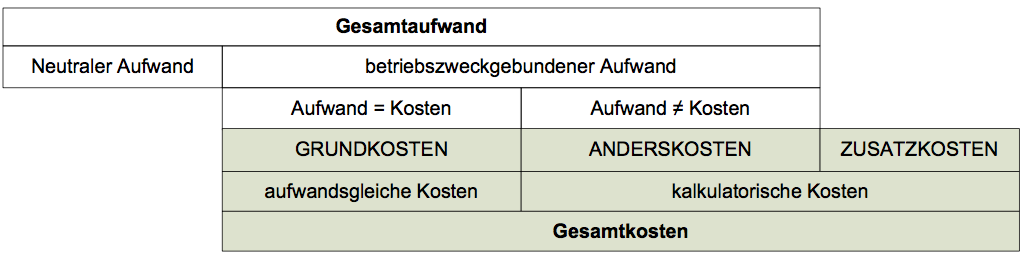
\includegraphics[width=\textwidth]
	{kapitel/gruppe4_2/bilder/abgrenzung_aufwand}
	\caption{Abgrenzung Aufwand - Kosten, nach Handbuch der Kostenartenrechnung 2005}
	\label{fig_abgrenzung_aufwand}
\end{figure}

In der Betrachtung der primären und sekundären Kostenarten, sind in einer Hochschule die sekundären Kostenarten besonders interessant, da sie die Kosten der Bereiche zusammenfassen und einen Überblick verschaffen.

Wie das Beispiel der Abbildung \ref{fig_uebergang_primaerkosten} zeigt, bauen sich die sekundären Kosten, in der Kostenstellenrechung, durch das Zusammenfließen der primären Kosten auf. An der Leibnitz Universität Hannover (LUH) wurden, für das SAP-System, 900 Primärkostenarten in 140 Sekundärkostenarten verdichtet und zugeordnet.\footnote{\cite{pkl_2005}}

\begin{figure}[h!]
	\centering
	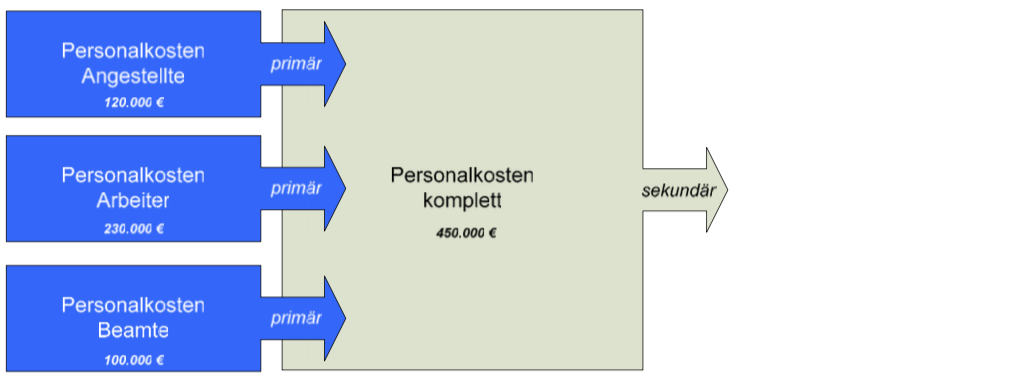
\includegraphics[width=\textwidth]
	{kapitel/gruppe4_2/bilder/uebergang_primaerkosten}
	\caption{Übergang von Primär- in Sekundärkosten,\\nach Handbuch der Kostenartenrechnung 2005}
	\label{fig_uebergang_primaerkosten}
\end{figure}

Diese Primärkostenarten und Sekundärkostenarten sind im Jahr 2005 im Rahmen des Projektes “Uni2001” für ganz Niedersachsen abgestimmt worden und im SAP-System eingepflegt. Ein entsprechender Abgleich mit Mitarbeitern der Hochschule Emden/Leer für die vorhandenen und besonders der genutzten Kostenarten sollte bei der konkreten Projektplanung unbedingt erfolgen. Die Hierarchie der Kostenarten der Hochschule sollten sich ähnlich, wenn nicht sogar gleich, dem Beispiel der Abbildung \ref{fig_kostenartenhierarchie_uni2001} der LUH darstellen.

\begin{figure}[h!]
	\centering
	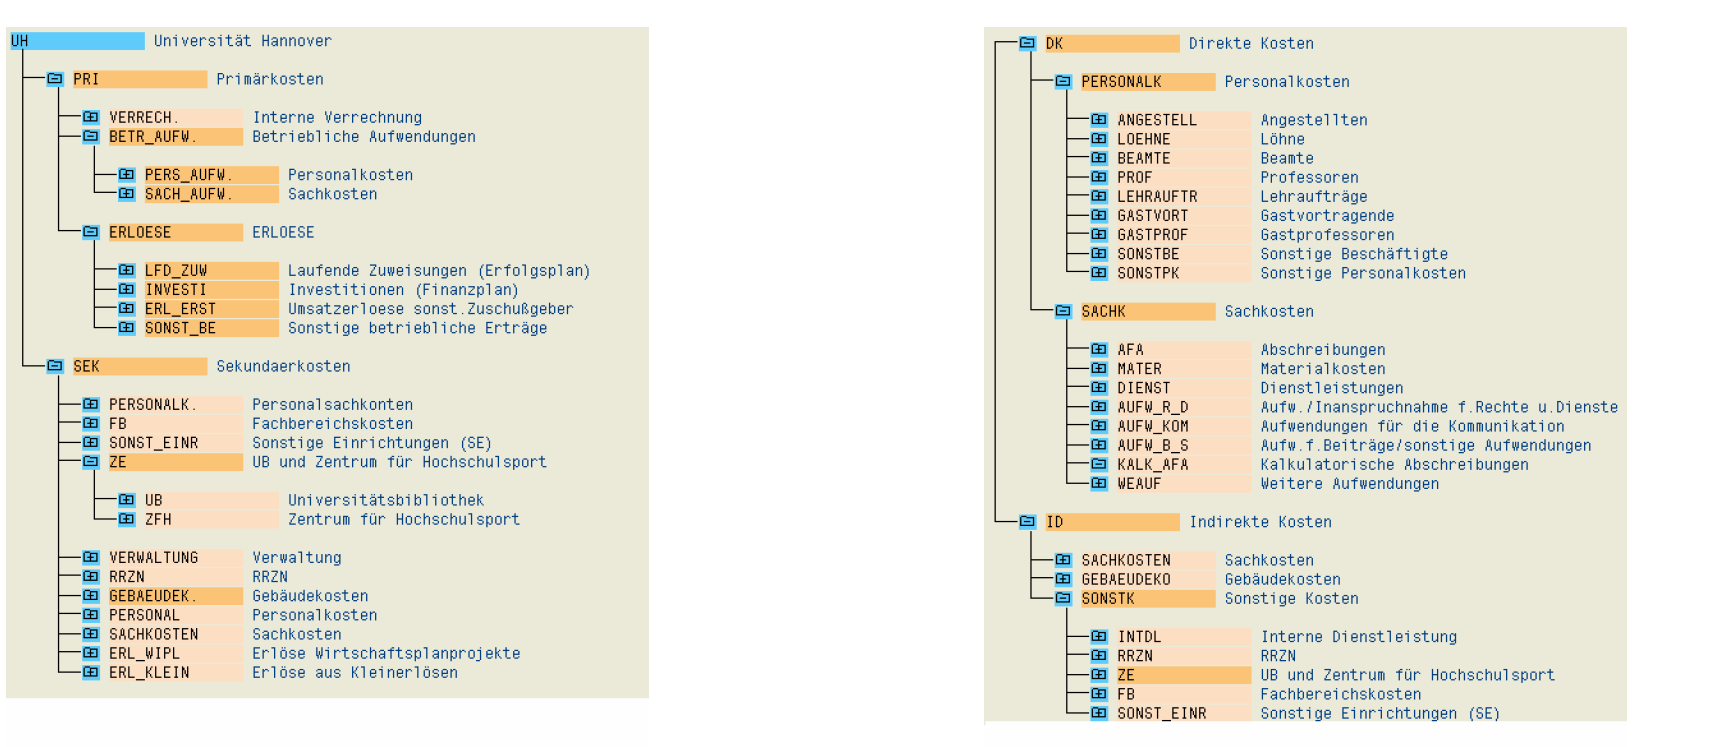
\includegraphics[width=\textwidth]
	{kapitel/gruppe4_2/bilder/kostenartenhierarchie_uni2001}
	\caption{Kostenartenhierarchie der Hochschulen Uni2001,\\nach Handbuch der Kostenartenrechnung 2005}
	\label{fig_kostenartenhierarchie_uni2001}
\end{figure}
% !TEX root = ../../../main.tex
% !TEX encoding = UTF-8 Unicode
% !TEX encoding = UTF-8

\subsection{Kostenarten in der IT}
In einer Hochschule ist ein Rechenzentrum für die Aufgaben der IT zuständig.
Der Rechenzentrumsleiter ist in einem Netzwerk, aus leitenden Personen der Hochschule, das Zentrum der personellen IT-Komponenten. In der IT einer Hochschule werden direkte Kosten zwischen den Primärkategorien Hard- und Software, operativer Betrieb und Verwaltung differenziert.\footnote{\autocite[494]{hansen_business_2009}}

Zusätzlich ist ein Rechenzentrum der Hochschule, nach Interview-Aussage des Rechenzentrumsleiters der Hochschule Emden/Leer, jährlich auf ein bestimmtes Budget festgelegt. Danach ist die Tabelle \ref{tab_auswahl_IT_kostenarten}\footnote{\autocite[493-498]{hansen_business_2009}} zu beachten, welche Kosten budgetiert sind und welche nicht. Die folgenden Tabellen sind für den Rechenzentrumsleiter als Kontrollhilfe angedacht, damit keine IT-Kostenarten unbeachtet bleiben.

\begin{table}[h!]
	\begin{tabularx}{\textwidth}{|X|X|}
		% Überschriften
		\hline \textbf{Budgetierte Kosten}  &  \textbf{Nicht budgetierte Kosten}\\
		% Zeile 1
		\hline Software-Entwicklung 
			\begin{itemize}
				\item Neuentwicklung und Anpassungen
				\item Personal- und Sachkosten	
			\end{itemize}  
		& Negative Produktivitätseffekte
			\begin{itemize}
				\item Antwort-, Rüst- und Bearbeitungszeit
				\item Motivation
				\item Ergonomie
			\end{itemize} \\ 
		% Zeile 2	
		\hline Kommunikation \begin{itemize}
			\item Netzwerk
			\item Personal- und Sachkosten			
		\end{itemize} & Ausfall \begin{itemize}
			\item geplant
			\item ungeplant
		\end{itemize} \\ 
		% Zeile 3
		\hline Hardware / Software \begin{itemize}
			\item Abschreibung, Miete und Leasing
			\item Entsorgung
			\item Client / Server
			\item Administration	
		\end{itemize} & Endbenutzer \begin{itemize}
			\item Peer-Support (selbst/gegenseitig)
			\item Unproduktives Konfigurieren
			\item Qualifizierung (selbst /gegenseitig)
		\end{itemize}  \\
		% Zeile 4
		\hline Support &   \\
		% Zeile 5 
		\hline Systembetrieb und Systemmanagement & \\
		\hline
	\end{tabularx}
	\caption{Auszug der IT-Kostenarten nach Krcmar}
	\label{tab_auswahl_IT_kostenarten}
\end{table}

\clearpage 

Als spezielle IT-Kostenarten werden von Gadatsch und Mayer aufgelistet\footnote{\autocite[349]{gadatsch_masterkurs_2014}}:

\begin{table}[h!]
	\begin{tabularx}{\textwidth}{|l|X|}
		% Überschriften
		\hline \textbf{Sekundäre Kostenarten}  &  \textbf{Primäre Kostenarten}\\
		% Zeile 1
		\hline Hardware-Kosten &
		\begin{itemize}
			\item Miete / Leasing
			\item Hardware
			\item Leitungsgebühren
			\item Wartung
		\end{itemize} \\ 
		% Zeile 2	
		\hline Software-Kosten  & 
		\begin{itemize}
			\item Miete / leasing
			\item Software
			\item eigene Entwicklung
			\item Externe Wartung
			\item Beratung
		\end{itemize} \\ 
	% Zeile 3
	\hline Daten-Kosten &
	\begin{itemize}
		\item Beratung
		\item Kauf
	\end{itemize}  \\
	% Zeile 4
	\hline Sonstige IT-Kosten &
		\begin{itemize}
			\item IT-Verbrauchsmaterial
			\item IT-Versicherungen
			\item Beiträge zu Fachverbänden
			\item IT-Fachliteratur
			\item IT-Schulungen
		\end{itemize}\\
	% Zeile 5 
	\hline Innerbetriebliche IT-Leistungsverrechnung & 
	\begin{itemize}
		\item Umlagen
		\item Entwicklungskosten
		\item Benutzerservice
	\end{itemize}\\
	\hline
\end{tabularx}
\caption{Auflistung der speziellen IT-Kosten, nach Gadatsch \& Mayer}
\label{tab_auflistung_spezielle_IT_Kosten}
\end{table}

Die Kostenarten aus den Auflistungen der Tabellen \ref{tab_auswahl_IT_kostenarten} und \ref{tab_auflistung_spezielle_IT_Kosten} eignen sich laut Hansen\footnote{\autocite[493-498]{hansen_business_2009}} für die Betrachtung der Kosten an einer Hochschule.

Als mögliche Nutzung der Kostenarten, schlägt Krcmar die TCO-Methode als Bewertungstechnik vor, was ausführlicher im Kapitel \ref{kosten_zeit_anwendung} beschrieben und zur Teilkalkulation verwendet wird.\footnote{\autocite[144]{krcmar_einfuhrung_2015}} Die TCO-Methode nutzt die Kostenarten, um die wirtschaftlichen Auswirkungen in der IT aufzuzeigen.

\clearpage

Vor allem im Bezug auf Kostenarten und IT wird als Trend ein IT-Controller empfohlen\footnote{\autocite[49]{gadatsch_masterkurs_2014}}, um eine erfolgreiche Wertschöpfung in der IT zu erreichen. Der IT-Controller hat die Transparenzverantwortung gegenüber dem CIO und entlastet ihn damit, wodurch der CIO sich gezielt auf seine Entscheidungsverantwortung konzentrieren kann.\footnote{\url{http://vfhinf.oncampus.de/loop/Zusammenarbeit_zwischen_CIO_und_IT-Controller}} Sollte die Hochschule Emden/Leer dieser Empfehlung folgen, ist besonders auf die klare Rollenverteilung zwischen CIO und IT-Controller zu achten. Ihre Kompetenzen dürfen sich nur in Ausnahmen gegenseitig blockieren. Der CIO sollte im Zweifel eine Entscheidungsgewalt haben und passend dazu die Konsequenzen alleine tragen, wenn er die Entscheidungsgewalt nutzt. Im idealen Fall tragen Beide die endgültige Entscheidung in einem Kompromiss.

Gerade in einem solch zentralen Projekt, mit hohem Anteil an IT-lastigen Themen, ist es zumindest empfehlenswert über einen IT-Controller nachzudenken.\footnote{\autocite[11-15]{stratmann_it_2013}} Besonders ist hier auch die höhere Komplexität zu beachten, die jeweils in der IT, DFG geförderter Referenzprojekte, entstand. Einige Referenzprojekte werden später im Kapitel \ref{section_projekt_beispiele} vorgestellt und mit der Hochschule Emden/Leer verglichen. Doch zuvor sollen im Kapitel \ref{section_verfahren_schaetzung} ausgewählte Kosten- und Zeitschätzungen erläutert werden, wie die empfohlenen Kostenarten in der Kalkulation Verwendung finden.











\section{Verfahren für die Kosten- und Zeitschätzung}
\label{section_verfahren_schaetzung}
Nachdem in Kapitel \ref{section_kostenarten} die für diese Arbeit relevanten Kostenarten beleuchtet wurden, werden in diesem Kapitel Möglichkeiten aufgezeigt, um die Kosten und die zur Realisierung benötigte Zeit zu schätzen. Im weiteren Verlauf werden Planungs- und Überwachungsinstrumente des Projektmanagements erläutert, die für das durchzuführende Projekt am geeignetsten scheinen. Dabei liegt der Fokus vor allem auf einer möglichst agilen Umsetzung des Projekts. Abschließend werden die untersuchten Verfahren beispielhaft auf drei konkrete Komponenten des Projekts angewendet.

% !TEX root = ../../../main.tex
% !TEX encoding = UTF-8 Unicode
% !TEX encoding = UTF-8

\subsection{Projektmanagement an einer Hochschule}
\label{subsection_projektmanagement_hochschule}
Wie bereits in Kapitel \ref{chapter_grundlagen_INM} beschrieben, weißt eine Hochschule als Organisation eine Reihe von Besonderheiten auf. Für das Projektmanagement bedeutet besonders die Tatsache, dass die einzelnen Fachbereiche ein hohes Maß an Autonomie und Entscheidungskompetenzen besitzen, eine entsprechend angepasste Herangehensweise.\footnote{\cite{hansen_business_2009}}

Die zentrale Herausforderung des Projektmanagements ist es, die Interessen der unterschiedlichen Verwaltungsbereiche, der späteren Nutzer und der Hochschulleitung zu wahren und zu vereinen. Durch die Autonomie der Fachbereiche und deren unterschiedlichen Interessen ist es möglich, dass sich innerhalb der Hochschule konkurrierende Arbeitsgruppen bilden. Es ist daher eine weitere, nicht zu unterschätzende, Aufgabe des Projektmanagements, die Kommunikation zwischen allen beteiligten Arbeitsgruppen, möglichen externen Akteuren und dem akademischen Bereich aufrecht zu erhalten und zu fördern.\footnote{\cite{altvater_organisation_2007}}

Des Weiteren führen umfangreiche Änderungen in Organisationen oftmals zu einer besonderen Eigendynamik, die, im Zusammenspiel mit den aufgeführten Besonderheiten einer Hochschule, zu nicht kalkulierbaren oder unvorhersehbaren Geschehnissen führen können. Der Umstand, dass zu Projektbeginn in der Regel noch nicht alle, für eine exakte Planung benötigten, Informationen zur Verfügung stehen, erschwert zusätzlich die zufriedenstellende Organisation des Projektverlaufs. Um dem entgegen zu wirken ist es empfehlenswert, dass Projekt in iterativ-reflexiven Schleifen mit ausreichender Flexibilität durchzuführen.\footnote{\cite{hansen_business_2009}}

Durch die gewonnene Flexibilität sind Anpassungen während der Ausführung des Projektes möglich und auf besondere Befindlichkeiten kann eingegangen werden. Durch eine iterative Durchführung wird außerdem dem Vorhaben Rechnung getragen, dass nach jeder Umsetzung einer Komponente über den weiteren Verlauf des Projekts reflektiert werden kann.


\subsection{Kostenschätzung (Total Cost of Ownership)}
\label{subsection_kostenschatzung_TCO}
Neben der Organisation und Durchführung des Projekts bildet die Schätzung der Kosten im Vorfeld eine weitere wichtige Säule des Projektmanagements. Eine möglichst ganzheitliche und realistische Erfassung aller potentiell entstehenden Kosten ist dabei notwendig, um die Entscheidung für oder gegen ein Projekt anhand fundierter Informationen treffen zu können.

Das Total-Cost-Of-Ownership-Konzept wurde im Rahmen einer Studie der Gartner Group zur vollständigen Erfassung der direkten und indirekten Kosten eines PC-Arbeitsplatzes entwickelt. Das Ergebnis der Studie hat dabei gezeigt, dass nur ca. 20\% der Gesamtkosten tatsächlich auf die direkten Anschaffungskosten von Hard- und Software entfallen. Der Großteil der entstehenden Kosten wird folglich durch den Einführungsprozess neuer Systeme und den langfristigen Betrieb selbiger verursacht. Der Einsatz der TCO-Methode kann demnach dabei helfen, ein Bewertungsobjekt mit allen zugehörigen, kostenverursachenden Aspekten zu erfassen und zu bewerten.\footnote{\cite{hansen_business_2009}}

Die Tatsache, dass es sich bei dem untersuchten Studienobjekt lediglich um einen “wenig komplexen” PC-Arbeitsplatz handelt, lässt vermuten, dass bei Einführung komplexer Systeme (z.B. Dokumentenmanagement) der Anteil der Anschaffungskosten über den gesamten Lebenszyklus des Systems weiter schrumpft, während beispielsweise Inbetriebnahme, Wartung und Schulung wesentlich mehr Kosten verursachen. Dieser Zusammenhang verdeutlicht die Wichtigkeit der ganzheitlichen Kostenbetrachtung und rechtfertigt den Einsatz des TCO-Konzepts, welches es zum Ziel hat, den Vollständigkeitsgrundsatz der Kostenrechnung\footnote{\cite{grob_einfuhrung_2004}} zu erfüllen.

Grundsätzlich wird im Rahmen der TCO-Aanalyse zwischen direkten und indirekten, bzw. budgetierten und nicht-budgetierten, Kosten unterschieden. In die Kategorie der direkten Kosten fallen dabei alle Investitionen, die zur Beschaffung und Bereitstellung der IT-Komponente notwendig sind. Die Bezeichnung als budgetierte Kosten liegt darin begründet, dass selbige einem konkreten Bereich (z.B. Hochschulrechenzentrum bei Anschaffung eines neuen Servers) zugeschrieben werden können. Im Gegensatz dazu handelt es sich bei indirekten Kosten um Ausgaben, die außerhalb des Bereichs auftreten, der die direkten Kosten zu tragen hat, wodurch sie keinem konkreten Budget zugeschrieben werden können. Eine generische Übersicht der direkten und indirekten Kategorien zeigt Abbildung \ref{fig_generische_kostenarten} \footnote{\cite{hansen_business_2009}}.

\begin{figure}[h!]
	\centering
	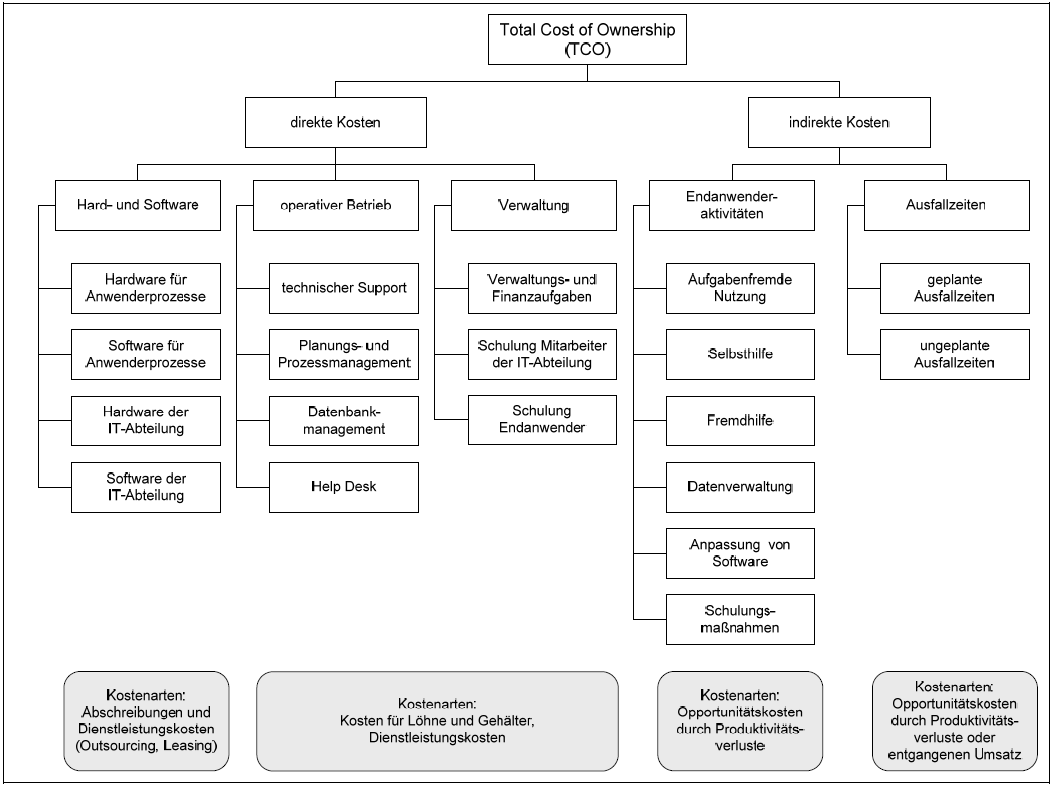
\includegraphics[width=10cm]{kapitel/gruppe4_2/bilder/generische_kostenkategorien}
	\caption{generische Kostenkategorien und -arten, nach Hansen}
	\label{fig_generische_kostenarten}
\end{figure}

Während die im Diagramm dargestellten direkten Kosten auch direkt in der IT-Abteilung anfallen und nachvollziehbar, beziehungsweise durch angemessenen Aufwand berechenbar, sind, entstehen die indirekten Kosten in der Regel durch Endanwender und deren “unsachgemäße Nutzung” der bereitgestellten Infrastruktur. Dies ist theoretisch bereits dann der Fall, wenn ein Mitarbeiter einen anderen Mitarbeiter bei der Lösung von IT-Problemen unterstützt, obwohl dies nicht seine eigentliche Aufgabe ist. Durch diese Arbeiten außerhalb seines Zuständigkeitsbereichs werden die eigentlichen Kernaktivitäten des Mitarbeiters vernachlässigt, wodurch seine Produktivität sinkt. Dieser Produktivitätsverlust wird durch sogenannte Opportunitätskosten abgebildet und als indirekten Kosten erfasst.

Die Erhebung der Informationen, die notwendig sind, um indirekte Kosten beziffern zu können, kann sich jedoch als äußerst schwierig und zeitaufwendig herausstellen. Aufgrund fehlender formalisierter Techniken zur Erfassung eben dieser Positionen, empfiehlt die Gartner Group den Einsatz von Befragungen und Fokusgruppen, was neben dem bereits erwähnten, hohen zeitlichen Aufwand, außerdem zu Problemen hinsichtlich der Validität der Daten führen kann.\footnote{\cite{hansen_business_2009}}

Ferner besteht die Gefahr, dass durch die Berücksichtigung von Opportunitätskosten der in Kapitel \ref{subsection_projektmanagement_hochschule} beschriebene, notwendige Austausch und Kontakt zwischen verschiedenen Arbeitsgruppen und Fachbereichen stark eingeschränkt wird. Deshalb sollte in diesem speziellen, nicht-industriellen, Fall einer Hochschule auf die initiale Berücksichtigung der indirekten Kosten verzichtet werden. Im späteren Projektverlauf, nachdem das Zusammenspiel aller Akteure etabliert und gefestigt ist, muss jedoch versucht werden, diese Daten zu evaluieren und in die Kalkulation mit einzubeziehen.

Eine beispielhafte Kalkulation auf Grundlage der TCO-Methode der Gartner Group wird in Kapitel \ref{subsubsection_dokusystem_alfresco} durchgeführt. Als unterstützende Software zur Berechnung dient die kostenlose Anwendung TCO-Tool.\footnote{\url{http://sourceforge.net/projects/tcotool/}}
\subsection{Zeitplanung}
Neben der Einschätzung der zu erwarteten Kosten soll der zeitliche Ablauf der einzelnen Projektkomponenten beleuchtet werden. Die aufsummierte Dauer der einzelnen Komponenten ergibt dann den gesamten zeitlichen Aufwand Projekts. Zur zeitlichen Planung der erforderlichen Schritte, sowie der Ablaufplanung einzelner Arbeitspakete werden Gantt-Diagramme eingesetzt. Die Anwendung eines solchen Gantt-Diagramms stellt das erste Kapitel dieses Abschnitts dar. Die Einhaltung der zuvor definierten Meilensteine und Arbeitsschritte wird dabei anhand der Meilensteintrendanalyse durchgeführt. Wie die Meilensteintrendanalyse zur Überwachung der Projektmodule eingesetzt werden soll wird im zweiten Teil dieses Kapitels erklärt. 

\clearpage
\section{Ausgewählte Projekt-Beispiele - KL}
\textit{Autor: Klaus Landsdorf}

\label{section_projekt_beispiele}
Die DFG hatte im Bezug auf die Förderung in jedem Durchgang die vier besten Projekte ausgewählt.
Diese wurden mit 50.000 EUR für die detaillierte Planungsphase und deren Umsetzung ausgestattet.
In einem zweiten Förderzeitraum, von maximal 5 Jahren, wurden zwei der vier Projekte mit jeweils 250.000 EUR pro Jahr ausgestattet.
Insgesamt entspricht das einem Fördervolumen von gut 1,3 Mio. EUR für ein integriertes Informationsmanagement.
Die folgenden Projekte wurden im Zeitraum 2005 - 2010 durchgeführt und haben ihre Erfahrungen in Publikationen bereitgestellt.\footnote{\cite{kerres_hochschulen_2005}}

Als Bestätigung dieser Zahlen weist die TU München mehr als fünfzig Mitarbeiterinnen und Mitarbeiter im Projekt aus. Zu ihrem integrierten Informationsmanagement bekam das Projekt insgesamt ca. 2,5 Mio. EUR. Die TU München stellte dazu selbst weitere Sondermittel aus dem Erneuerungsprojekt InnovaTUM zur Verfügung.\footnote{\cite{bode_informationsmanagement_2010}}

\subsection{Beispiele des integrierten Informationsmanagements}
Münster Information System for Research and Organization (MIRO) ist das integrierte Informationsmanagement an der Westfälischen Wilhelms-Universität  (WWU) Münster.

Die ersten Bemühungen starteten im Jahr 2003 und wurden in den folgenden Jahren vorangetrieben. Im Jahre 2005 wie zum abschließenden Berichtsstand der WWU 2013 existierten 15 Fachbereiche an der WWU. Die 130 Studienfächer sanken in diesem Zeitraum auf 110. Auch die ca. 39.000 Studierenden sind im Jahr 2013 auf ca. 37.000 Studierende gesunken. An der WWU waren zum Zeitpunkt der Antragstellung etwa 5.000 Personen beschäftigt, davon 600 Professoren, 2.600 wissenschaftliche und 1.800 weitere Mitarbeiter. Im Jahr 2013 sind über 550 Professoren und ca. 3800 wissenschaftliche Beschäftigte an der WWU.\footnote{\cite{vogl_bericht_2013}}

\begin{itemize}
	\item Erreichtes
	\begin{itemize}
		\item Flexible IT-Architektur - SOA / SOI
		\item Identitätsmanagement (MORITZ)
		\item Digitlaes Publizieren
		\item Enterprise Content Management (ECM) (Alfresco, SAN, Oracle Cluster)
		\item Mobile Dienste (Alfresco)
		\item Portalinfrastruktur (Apache Webserver, JBoss, Oracle Cluster)
	\end{itemize}
	\item Aufwand
	\begin{itemize}
		\item 16 wissenschaftliche Mitarbeiter - 8 davon DFG gefördert
		\item über einen Zeitraum von sechs Jahren
		\item Finanzmittel
		\begin{itemize}
			\item beträchtliche Finanzmittel durch das Rektorat der Universität
			\item vor allem notwendige Sachausgaben
		\end{itemize}
	\end{itemize}
\end{itemize}

\textit{„Nach über zehn Jahren ist festzuhalten, dass sich die Strukturen in der Informationsverarbeitung und -versorgung sehr bewährt haben. Den Verantwortlichen ist es gelungen, die Informationsverarbeitung und -versorgung in Münster auf einen beachtlichen Stand der Technik und Organisation zu bringen.“}\footnote{\cite{bode_informationsmanagement_2010}}

\todo[inline]{Tabelle neu formatieren}
\begin{table}[h!]
	\begin{tabularx}{\textwidth}{l|r}
		\hline
		\textbf{Kostenaufteilung Annahme MIRO} & \textbf{Betrag in EUR}\\
		Gesamtvolumen über 5 Jahre & 1.300.000\\
		Personalkosten IT ca. 75\% & 975.000\\
		Kosten pro Projektmitarbeiter (16) & 56.875 (ca. 5.080 / Monat)\\ 
		Sonstige Kosten (unbekannt) & 325.000 (ca. 65.000 / Jahr)\\
		\hline
    \end{tabularx}
    \caption{Annahme der minimalen Investition in Münster}
    \label{tab_minimale_investition_munster}
\end{table}

Die geschätzten Kosten der Projektmitarbeiter der Tabelle \ref{tab_minimale_investition_munster} passen zu den Angaben der DFG-Sätze 2015, worin ein/e Doktorandin/ Doktorand und Vergleichbare EUR 5.050 monatlich verdienen und Sonstige(r) wissenschaftliche(r) Mitarbeiterinnen oder Mitarbeiter EUR 4.250 Vergütung erhalten (vgl. Tabelle \ref{tab_ubersicht_lohne}) . Das Mittel von der Professur Vergütung bis zum angestellten Mitarbeiter liegt sogar etwas höher bei ca. EUR 5.240 monatliche Vergütung.

Die Angabe der Personalkosten von 75 \%  leitet sich aus einem Bericht der Kosten in fertigenden Unternehmen und der Automobilbranche ab.\footnote{\cite{schuelein_2009}}

Ein weiteres Projekt ist das „Karlsruher Integriertes InformationsManagement“ (KIM).
\begin{figure}[h!]
	\centering
	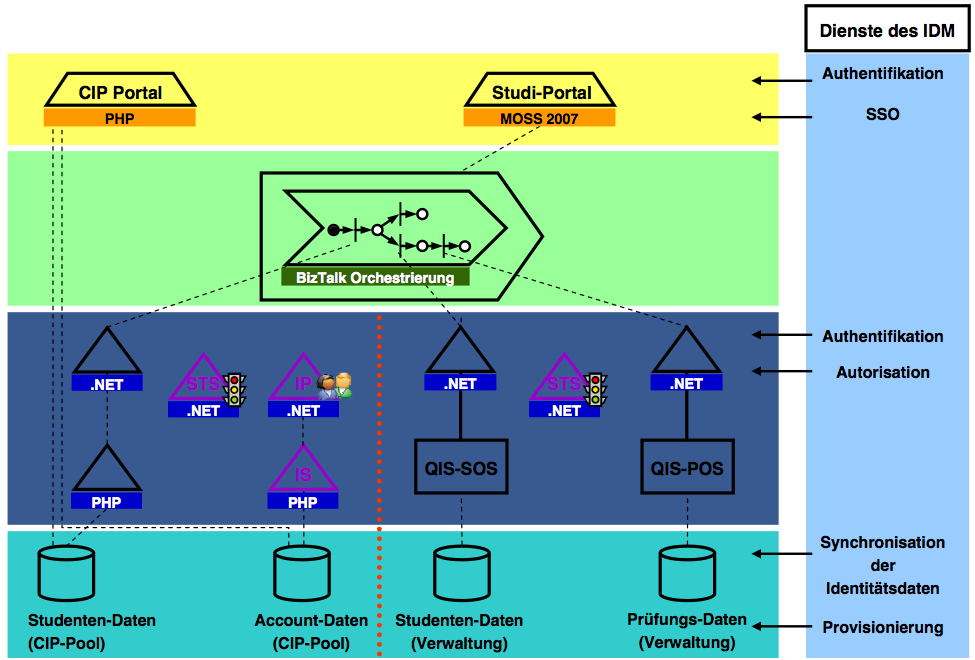
\includegraphics[width=\textwidth]
	{kapitel/gruppe4_2/bilder/ubersicht_karlsruhe}
	\caption{Erreichtes im Überblick für Karlsruhe, nach Juling Best Practice Workshop 2008}
	\label{fig_ubersicht_karlsruhe}
\end{figure}

KIM ist im Ansatz eine dienstorientierte Föderation, in der die jeweiligen Fachbereiche sich an bestimmte Schnittstellen halten und selbst die Dienste in ihrer bevorzugten Art und Programmierung zur Verfügung stellen. Dabei wurde ein hoch komplexes, aber nach eigenen Angaben sehr flexibles System, im Rahmen der 5 Jahre DFG Förderung, geschaffen.\footnote{\cite{bode_informationsmanagement_2010}}

An der Universität Karlsruhe studieren (Stand 02/2014) ca. 24.500 Studenten ca. 9500 Mitarbeiter davon 346 Professoren mit Einnahmen in Mio. EUR 795 wovon Drittmittel EUR 339 Mio. betragen. Die Landesmittel sind mit EUR 212 Mio. und die Bundesmittel mit EUR 349 Mio. angegeben.\footnote{\url{https://www.kit.edu/mediathek/print_forschung/Flyer_KIT_de.pdf}} Den CIO bilden Rektorat und Vorstand.

\begin{figure}[h!]
	\centering
	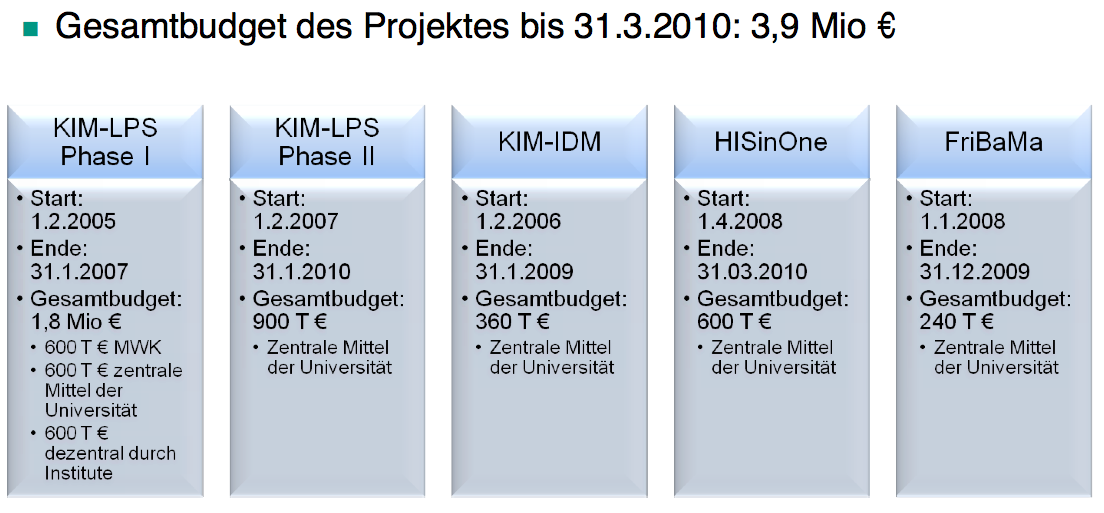
\includegraphics[width=\textwidth]
	{kapitel/gruppe4_2/bilder/uberblick_projekt_KIM}
	\caption{Erreichtes im Überblick für Karlsruhe, nach Juling Best Practice Workshop 2008}
	\label{fig_uberblick_projekt_KIM}
\end{figure}

Aus den bekannten Werten des Projektes MIRO kann nun abgeleitet werden, wieviele Personen an dem Projekt mitgewirkt haben könnten und welche Beträge für sonstige Kosten zur Verfügung standen. Diese Annahme in der Tabelle \ref{tab_minimale_investition_karlsruhe} ist rein fiktiv und dient lediglich dem Vergleich mit dem Projekt MIRO, dass den selben DFG-Förderungen gegenüber steht.

\todo[inline]{Tabelle neu formatieren}
\begin{table}[h!]
	\begin{tabularx}{\textwidth}{l|r}
		\hline
		\textbf{Kostenaufteilung Annahme KIM} & \textbf{Betrag in EUR}\\
		Gesamtvolumen über 5 Jahre & 3.900.000\\
		Personalkosten IT ca. 75\% & 2.925.000\\
		Kosten pro Projektmitarbeiter (50 möglich) & 58.500 (ca. 4.875 / Monat)\\ 
		Sonstige Kosten (unbekannt) & 975.000 (ca. 81.250 / Jahr)\\
		\hline
	\end{tabularx}
	\caption{Annahme der minimalen Investition in Karlsruhe}
	\label{tab_minimale_investition_karlsruhe}
\end{table}

Die Hochschule Emden/Leer ist mit 4.626 Studierenden eine kleine Hochschule, für die nun in Tabelle \ref{tab_kostenaufteilung_emden_MIRO} beispielhaft eine fiktive Annahme durch Teilung, aus den Werten des MIRO Projektes, gezeigt wird. Die Grundlage wäre das Minimum, dass dem MIRO Projekt durch seine DFG Förderung zukam.

\todo[inline]{Tabelle neu formatieren}
\begin{table}[h!]
	\begin{tabularx}{\textwidth}{l|r}
		\hline
		\textbf{Kostenaufteilung Annahme KIM} & \textbf{Betrag in EUR}\\
		Gesamtvolumen über 5 Jahre (fiktiv) & 169.000\\
		Personalkosten IT ca. 75\% & 126.750\\
		Kosten pro Projektmitarbeiter (2 möglich) & 63.375 (ca. 5.281 / Monat)\\ 
		Sonstige Kosten (unbekannt) & 42.250 (ca. 8.450 / Jahr)\\
		\hline
	\end{tabularx}
	\caption{Annahme der minimalen Investition in Emden; Basis gegenüber MIRO 13\%}
	\label{tab_kostenaufteilung_emden_MIRO}
\end{table}

Mit EUR 1,3 Mio. bekannten Projektmitteln, hat die Universität Münster mit ca. 37.000 Studierenden und Jahresmitteln von EUR 621 Mio. zu Emden mit EUR 36 Mio. Jahresmittel und ca. 5.000 Studierenden einen Vergleichsanteil, im Bezug auf die Anzahl der Studenten, von 13\%.

Sollte man in Emden den Wert des Projektes etwas besser bewerten, kann man die Grundlage für das Minimum aus dem KIM Projekt durch seine DFG Förderung plus die Zuwendungen durch Zentral Mittel der Universität kalkulieren. Damit würde dem Projekt ein finanzielles Volumen wie in Tabelle \ref{tab_kostenaufteilung_emden_KIM} zustehen.

\todo[inline]{Tabelle neu formatieren}
\begin{table}[h!]
	\begin{tabularx}{\textwidth}{l|X}
		\hline
		\textbf{Kostenaufteilung Annahme KIM} & \textbf{Betrag in EUR}\\
		Gesamtvolumen über 5 Jahre (fiktiv) & 169.000\\
		Personalkosten IT ca. 75\% & 126.750\\
		Kosten pro Projektmitarbeiter (2 möglich) & 63.375 (ca. 5.281 / Monat)\\ 
		Sonstige Kosten (unbekannt) & 42.250 (ca. 8.450 / Jahr)\\
		\hline
	\end{tabularx}
	\caption{Annahme der minimalen Investition in Emden; Basis gegenüber KIM 20\%}
	\label{tab_kostenaufteilung_emden_KIM}
\end{table}

Bei einem anzunehmenden Mittelwert von ca. EUR 4.916 für Personal in Emden, würde etwas mehr Geld für die Position Personal benötigt oder es wird eine weniger oder eine halbe Stelle angesetzt. Mit EUR 3,9 Mio. hat die Universität Karlsruhe mit ca. 25.000 Studierenden und Jahresmittel von EUR 795 Mio.  zu Emden mit EUR 36 Mio. Jahresmittel und ca. 5.000 Studierenden einen Vergleichsanteil, im Bezug auf die Anzahl der Studenten, von 20\%.